\documentclass[11pt]{article}

% --------------------
% PACOTES ESSENCIAIS
% --------------------
\usepackage[utf8]{inputenc}     % Codificação UTF-8
\usepackage[T1]{fontenc}        % Fonte com acentuação
\usepackage[brazil]{babel}      % Idioma português
\usepackage{amsmath, amssymb}   % Símbolos matemáticos
\usepackage{graphicx}           % Inserção de imagens
\usepackage{geometry}           % Margens personalizadas
\usepackage{fancyhdr}           % Cabeçalhos e rodapés
\usepackage{enumitem}           % Listas personalizadas
%\usepackage{physics}            % Notação física e matemática
\usepackage{hyperref}           % Links no PDF
\usepackage{multicol}           % Colunas (opcional)
\usepackage{xcolor}
\usepackage{siunitx}
\usepackage{comment}
\usepackage{amsthm}

\theoremstyle{definition}
\newtheorem{obs}{Observação}
\newtheorem{definicao}{Definição}
\newtheorem{exemplo}{Exemplo}


% --------------------
% CONFIGURAÇÕES
% --------------------
\geometry{a4paper, margin=2.5cm}

\pagestyle{fancy}
\fancyhf{}
\rhead{Triângulo de velocidades}
\lhead{Caio Magno Mendonça Nicácio}
\cfoot{\thepage}

\setlength{\parskip}{0.5em}
\setlength{\parindent}{0pt}

% --------------------
% INÍCIO DO DOCUMENTO
% --------------------
\begin{document}
	
	\begin{center}
		\Large\textbf{TRIÂNGULO DE VELOCIDADES} \\
		\normalsize
		Data: \today
	\end{center}
	
	\hrule
	\vspace{1em}
	
	\tableofcontents
	\newpage
	
	\section{Triângulo de velocidades}
	\label{sec:introducao}
	
	\begin{quote}
		Forma geométrica de expressar a equação vetorial que relaciona o movimento relativo com o movimento absoluto das partículas fluidas que percorrem o rotor de uma máquina de fluxo.
	\end{quote}
	
	A seleção conveniente do sistema de referência é de fundamental importância para o estabelecimento de equações algébricas. A depender do sistema, o escoamento pode ser tratado como transiente ou estacionário, conduzindo à ideia de que o movimento de uma partícula fluida $P$ seja referido a um sistema de coordenadas que, por sua vez, também esteja em movimento. A Figura \ref{fig:sistema-coordenadas} apresenta o \textbf{sistema relativo de coordenadas}, o qual combina movimentos de rotação e translação em relação a um sistema fixo, chamado \textbf{sistema absoluto}.
	\begin{figure}[h!]
		\centering
		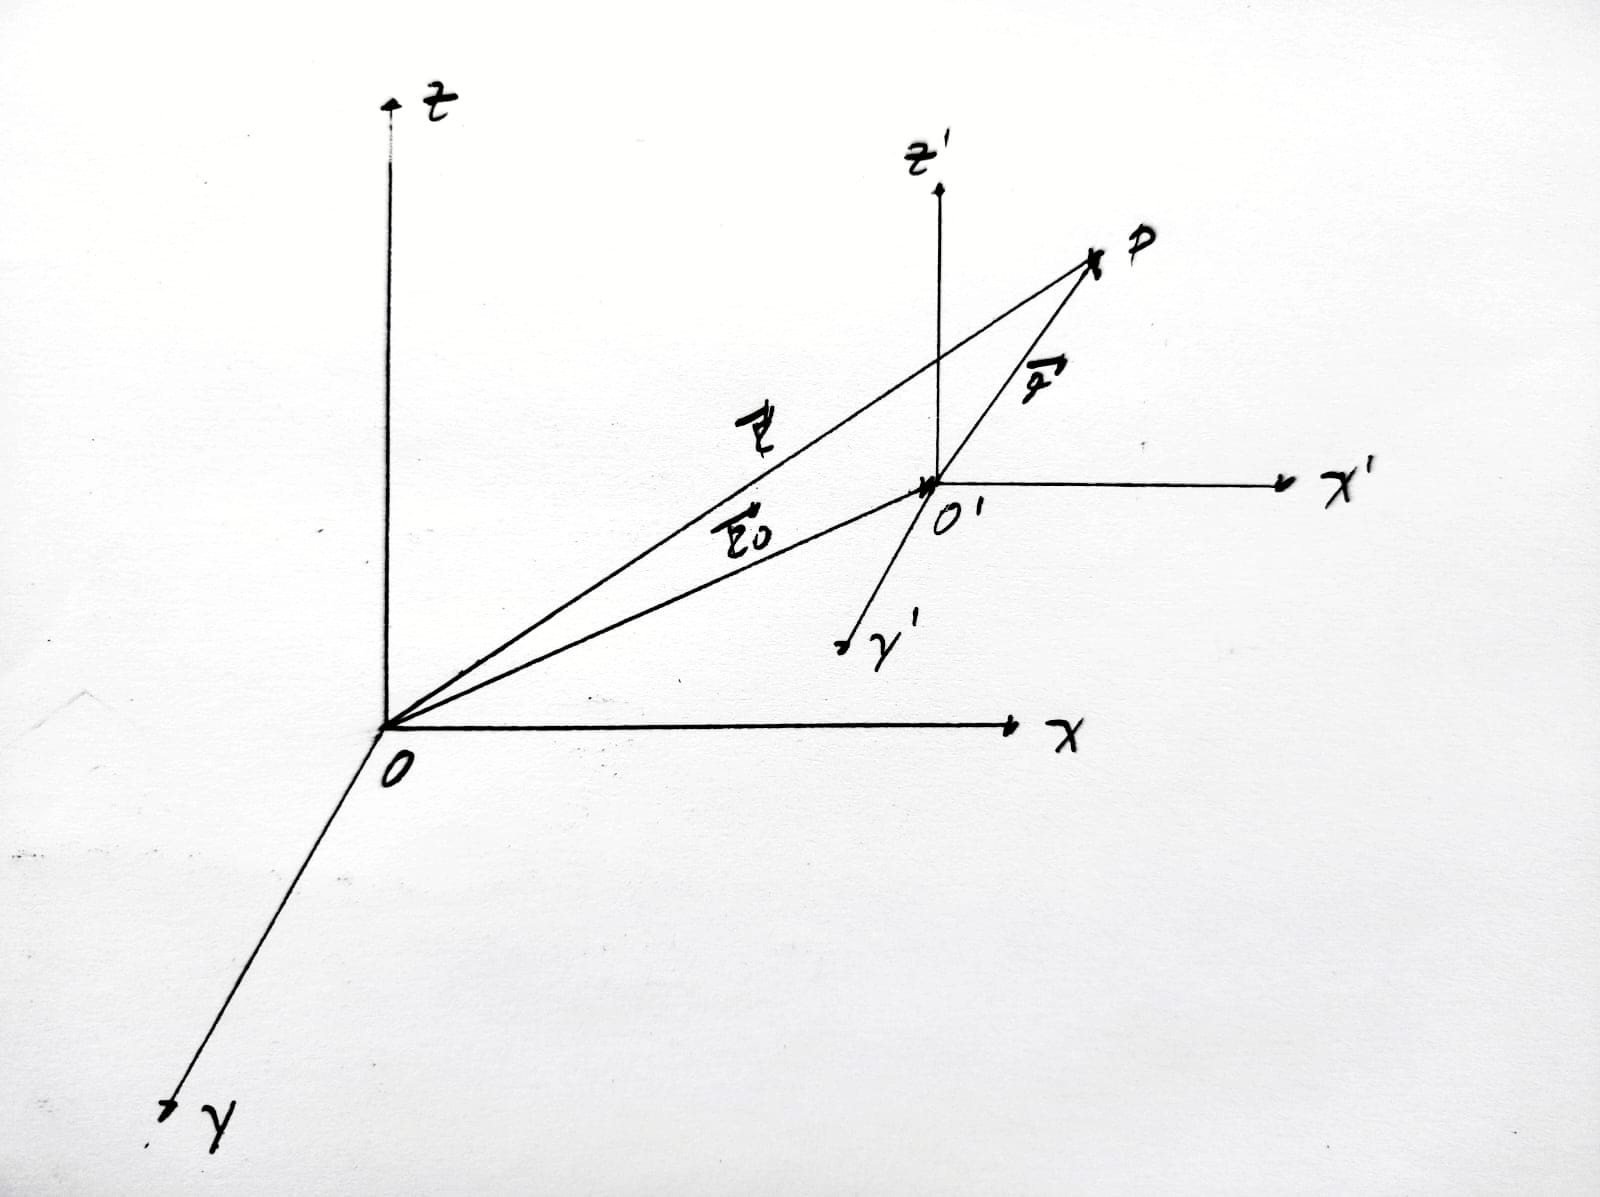
\includegraphics[width=0.48\textwidth]{figure/sistema-coordenadas.jpeg}
		%\captionsetup{width=16cm}
		\caption{\centering Sistema de coordenadas relativo ao sistema absoluto.}
		\label{fig:sistema-coordenadas}
	\end{figure}

	A relação entre os vetores posição nos dois sistemas é dada por
	\begin{equation}
		\boldsymbol{\vec{R}}=\boldsymbol{\vec{R}}_0+\boldsymbol{\vec{r}},
		\label{eq:vetor-posicao}
	\end{equation}
	onde $\boldsymbol{\vec{R}}$ é o vetor posição da partícula fluida $P$ em relação à origem do sistema absoluto; $\boldsymbol{\vec{R}}_0$ é o vetor posição da origem $O'$ em relação à origem dos sistema absoluto, $O$; $\boldsymbol{\vec{r}}$ é o vetor posição da partícula fluida $P$ com relação à origem $O'$ do sistema relativo.
	
	Designando-se os vetores unitários do sistema relativo de coordenadas por $\mathbf{i}'$, $\mathbf{j}'$ e $\mathbf{k}'$, e as componentes do vetor posição $\boldsymbol{\vec{r}}$ no sistema relativo por $x'$, $y'$ e $z'$, o vetor $\boldsymbol{\vec{r}}$ é expresso por
	\begin{equation}
		\boldsymbol{\vec{r}}=x'\, \mathbf{i}'+y'\, \mathbf{j}'+z'\, \mathbf{k}'.
		\label{eq:vetor-r}
	\end{equation}
	Derivando a Eq. \ref{eq:vetor-posicao} em relação ao tempo $t$, obtêm-se
	\begin{equation*}
		\boldsymbol{\vec{c}}=\frac{d\boldsymbol{\vec{R}}}{dt}=\frac{d\boldsymbol{\vec{R}}_0}{dt}+\frac{d\boldsymbol{\vec{r}}}{dt}.
	\end{equation*}
	As componentes escalares e os vetores unitários de $\boldsymbol{\vec{r}}$ variam em função do tempo. Logo,
	\begin{align}
		\frac{d\boldsymbol{\vec{r}}}{dt}&=\mathbf{i}'\, \frac{dx'}{dt}+x'\, \frac{d\mathbf{i}}{dt}+\mathbf{j}'\, \frac{dy'}{dt}+y'\, \frac{d\mathbf{j}}{dt}+\mathbf{k}'\, \frac{dz'}{dt}+z'\, \frac{d\mathbf{k}}{dt} \nonumber\\
		&=\mathbf{i}'\, \frac{dx'}{dt}+\mathbf{j}'\, \frac{dy'}{dt}+\mathbf{k}'\, \frac{dz'}{dt}+x'\, \frac{d\mathbf{i}}{dt}+y'\, \frac{d\mathbf{j}}{dt}+z'\, \frac{d\mathbf{k}}{dt} \nonumber\\
		\frac{d\boldsymbol{\vec{r}}}{dt}&=\mathbf{i}'\, \frac{dx'}{dt}+\mathbf{j}'\, \frac{dy'}{dt}+\mathbf{k}'\, \frac{dz'}{dt}+\boldsymbol{\vec{\omega}}\times\boldsymbol{\vec{r}}
	\end{align}
	Durante um intervalo infinitesimal $dt$, o corpo está sujeito a uma rotação infinitesimal $d\theta$. Logo, quando um corpo rígido sofre uma rotação $d\theta$ em torno de um eixo definido por um vetor unitário $\mathbf{n}$, a rotação é representada por
	\begin{equation*}
		d\boldsymbol{\vec{\theta}}=d\theta\,\mathbf{n},
	\end{equation*}
	ou seja, um vetor cuja direção é o eixo de rotação e cujo módulo é o ângulo infinitesimal $d\theta$ (Fig. \ref{fig:rotacao-1}).
	\begin{figure}[h!]
		\centering
		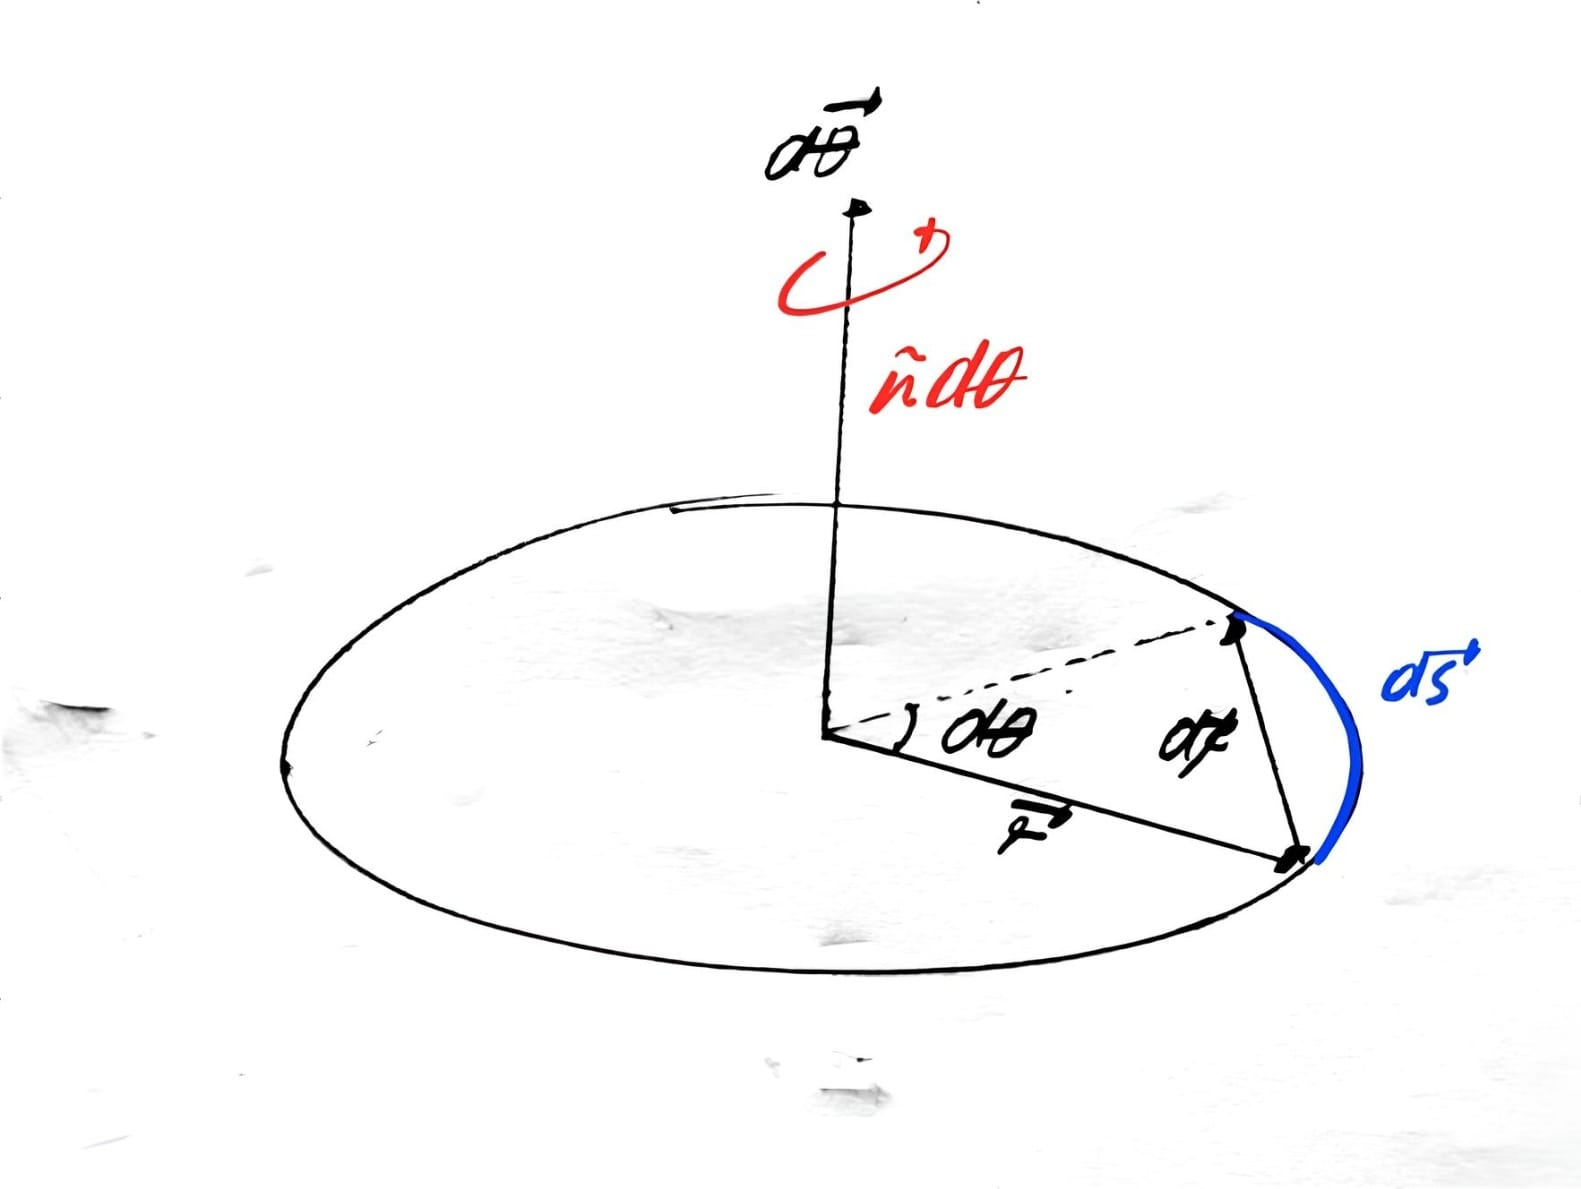
\includegraphics[width=0.48\textwidth]{figure/rotacao-1.jpeg}
		%\captionsetup{width=16cm}
		\caption{\centering Deslocamento linear infinitesimal $d\boldsymbol{\vec{r}}$ do vetor $\boldsymbol{\vec{r}}$ relativo a uma rotação $d\boldsymbol{\vec{\theta}}$.}
		\label{fig:rotacao-1}
	\end{figure}
	
	Conforme $d\theta \to 0$, $d\boldsymbol{\vec{S}}\to d\boldsymbol{\vec{r}}$, de modo que
	\begin{equation*}
		\frac{d\boldsymbol{\vec{S}}}{d\theta}=\boldsymbol{\vec{r}}\quad \therefore\quad \frac{d\boldsymbol{\vec{r}}}{d\theta}=\boldsymbol{\vec{r}}.
	\end{equation*}
	O vetor $d\boldsymbol{\vec{\theta}}$ é orientado ao longo do eixo instantâneo de rotação e, portanto, indica o plano de interação entre $d\boldsymbol{\vec{r}}$ e $\boldsymbol{\vec{r}}$, perpendicular a $d\boldsymbol{\vec{\theta}}$\footnote{A rotação ocorre em um plano fixo normal a $\mathbf{n}$.}.
	
	A variação infinitesimal da posição de $P$, $d\boldsymbol{\vec{r}}$ é perpendicular tanto a $\mathbf{n}$ quanto a $\boldsymbol{\vec{r}}$ e pode ser expressa vetorialmente como
	\begin{equation*}
		d\boldsymbol{\vec{r}}=d\boldsymbol{\vec{\theta}}\times \boldsymbol{\vec{r}}
	\end{equation*}
	\begin{figure}[h!]
		\centering
		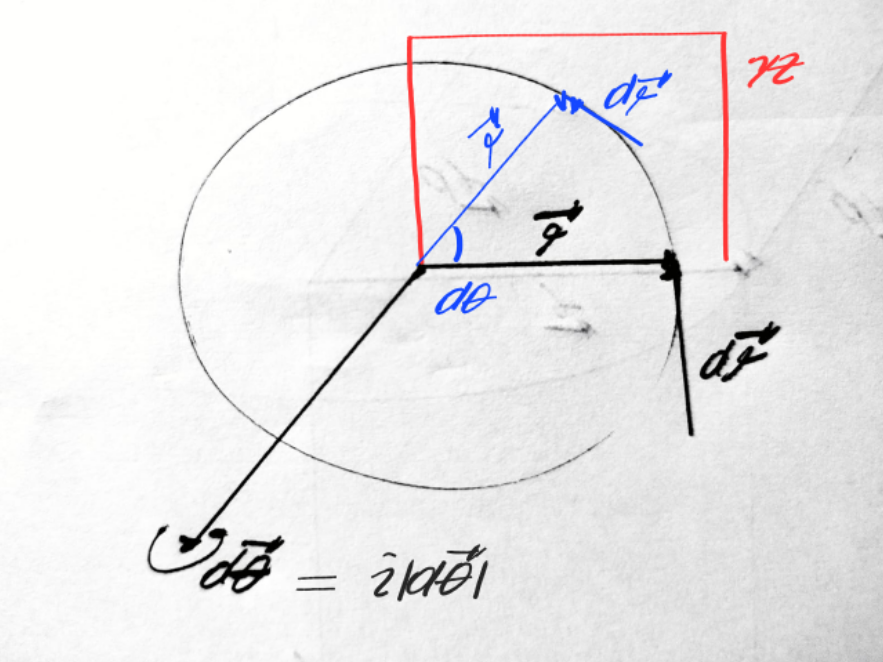
\includegraphics[width=0.48\textwidth]{figure/rotacao-2.png}
		%\captionsetup{width=16cm}
		\caption{\centering Deslocamento linear infinitesimal $d\boldsymbol{\vec{r}}$ do vetor $\boldsymbol{\vec{r}}$ relativo a uma rotação $d\boldsymbol{\vec{\theta}}$.}
		\label{fig:rotacao-2}
	\end{figure}
	
	\begin{comment}
		\begin{figure}[h!]
			\begin{minipage}[b]{0.48\textwidth}
				\centering
				
\includegraphics[width=\textwidth]{figure/estado-geral-tensao-1.png}
				\\[-1ex]\small (a)
				\label{fig:estado-geral-1}
			\end{minipage}
			\hfill
			\begin{minipage}[b]{0.48\textwidth}
				\centering
				
\includegraphics[width=\textwidth]{figure/estado-geral-tensao-2.png}
				\\[-1ex]\small (b)
				\label{fig:estado-geral-2}
			\end{minipage}
			\centering
			%\captionsetup{width=16cm}
			\caption{\centering Representação do estado geral de tensões em um ponto $Q$: (a) no sistema de coordenadas original e (b) no sistema resultante de uma rotação em relação ao sistema inicial.}
			\label{fig:estado-geral}
		\end{figure}
	\end{comment}
	
	\begin{comment}
		\begin{figure}[h!]
			\centering
			
\includegraphics[width=5.5cm]{figure/forca-plano-1.png}
			%\captionsetup{width=16cm}
			\caption{\centering Força $\boldsymbol{\vec{F}}$ aplicada em uma dada superfície.}
			\label{fig:forca-plano-1}
		\end{figure}
	\end{comment}
	
	
	%\bibliography{pos-textuais/referencias.bib}

\end{document}